\question{\bfseries Stable Molecule}

\subsection*{\sectionfont\upshape Background}

ในห้องปฏิบัติการวิจัยเคมีแห่งหนึ่ง\; คุณกุ้งกำลังศึกษาโครงสร้างของโมเลกุลชนิดหนึ่ง\;
ซึ่งประกอบไปด้วยอะตอมหลากหลายชนิดมาประกอบกันด้วยพันธะที่เชื่อมระหว่างอะตอมบางคู่ จนมีโครงสร้างเป็นกราฟต้นไม้

กล่าวคือโครงสร้างโมเลกุลนี้จะประกอบด้วยอะตอมทั้งสิ้น $N$ ชนิด ชนิดละ 1 อนุภาค (เรียกสั้น ๆ ว่า “ลูก”) 
และมีพันธะทั้งสิ้น $N-1$ พันธะที่เชื่อมอะตอมเหล่านี้เข้าด้วยกัน 
(เราจะเรียกอะตอมแต่ละลูกว่าลูกที่ $i$ สำหรับ $i = 1, 2, \ldots, N$)

คุณกุ้งสามารถกำหนดค่ามวลของอะตอมแต่ละลูกได้ โดยที่มวลของอะตอมลูกที่ $i$ จะกำหนดด้วยตัวแปร $m_i$ 
ซึ่งเป็นจำนวนเต็มบวก กล่าวคือมีเงื่อนไขว่า $m_i \geq 1$

โครงสร้างโมเลกุลนี้จะ \textbf{“เสถียร”} ก็ต่อเมื่อ แรงดึงดูดระหว่างอะตอม 2 ลูกที่เป็นพันธะต่อกันจะมีค่าไม่เกิน $P$ 
โดยแรงดึงดูดระหว่างมวลสามารถคำนวณได้จากผลคูณของมวลของอะตอมแต่ละลูก (นั่นแปลว่า $m_u \times m_v \leq P$ สำหรับทุกคู่อะตอม $u$ และ $v$ ที่มีพันธะต่อกัน)

\bigskip\noindent
\textbf{\uline{ตัวอย่าง}} 
เมื่อพิจารณาโครงสร้างโมเลกุลที่เกิดจากอะตอม 4 ลูกที่เชื่อมกันดังรูปทาง\ifpageodd{ขวา}{ซ้าย} 
และกำหนดให้ $P=12$ แล้วพบว่าโครงสร้างโมเลกุลรูปบนจะเสถียร แต่โครงสร้างอันล่างจะไม่เสถียร
\marginnote[-15\baselineskip]{%
    \centering
    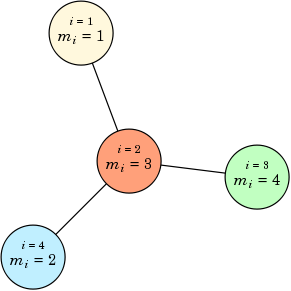
\includegraphics[width=0.97\linewidth]{figures/coding_national_stablemolecule_01.png}

    \bigskip\bigskip
    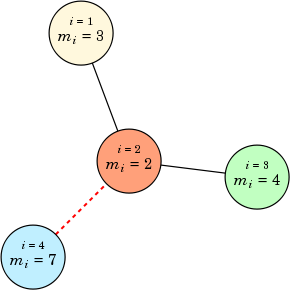
\includegraphics[width=0.97\linewidth]{figures/coding_national_stablemolecule_02.png}
}

\subsection*{\sectionfont\upshape Problem Statement}

จงเขียนโปรแกรมเพื่อรับข้อมูลที่กำหนดโครงสร้างโมเลกุล และค่าขีดจำกัดสูงสุดของแรงดึดดูดระหว่างอะตอม $P$ 
แล้วหาว่าคุณกุ้งจะสามารถกำหนดค่ามวลให้แก่อะตอมแต่ละลูกให้แตกต่างกันได้ทั้งหมดกี่รูปแบบ โดยที่โมเลกุลจะยังเสถียรอยู่

\subsection*{\sectionfont\upshape Program Specification}

โปรแกรมที่คุณเขียนจะต้องอ่านข้อมูลจาก stardard input 
และเขียนคำตอบลง standard output โดยข้อมูลจะมีฟอร์แมตดังต่อไปนี้

\bigskip\noindent
{\sectionfont\bfseries Input Format}
\begin{itemize}
\item บรรทัดที่ 1: มีจำนวนเต็มสองจำนวน $N$ และ $P$ คั่นด้วยช่องว่าง
\item อีก $N-1$ บรรทัดถัดมา บรรทัดที่ $j+1$ จะมีจำนวนเต็ม $u_j$ และ $v_j$ 
    คั่นด้วยช่องว่าง ซึ่งระบุว่ามีพันธะระหว่างอะตอมลูกที่ $u_j$ และอะตอมลูกที่ $v_j$  
\begin{lstlisting}
N P
u_1 v_1
u_2 v_2 <%\SuppressNumber\AlternateNumber{...}%>
        <%\AlternateNumber{N+1}%>
u_N v_N <%\ReactivateNumber%>
\end{lstlisting}
\textbf{หมายเหตุ:} กำหนดให้ $1 \leq u_j, v_j \leq N$ และ $u_j \neq v_j$
\end{itemize}

\medskip\noindent
{\sectionfont\bfseries Output Format}
\begin{itemize}
\item คำตอบประกอบด้วยจำนวนเต็ม 1 ตัว 
    ระบุจำนวนรูปแบบของโมเลกุลที่คุณกุ้งสามารถกำหนดมวลให้อะตอมแต่ละลูกได้ 
    โดยคำตอบจะต้องอยู่ในรูปของเศษที่เกิดจากการหารด้วย $1,\!000,\!000,\!007$
\end{itemize}

\subsection*{\sectionfont\upshape First Data Example}
\begin{tabular}{p{0.45\linewidth}p{0.45\linewidth}}
\toprule
Example Input & Example Output \\
\midrule
\ttfamily\setstretch{0.8}
4 2 \newline
1 2 \newline
2 3 \newline
4 2 &
\ttfamily\setstretch{0.8}
9 \\
\bottomrule
\end{tabular}

\medskip\noindent
\textbf{อธิบายตัวอย่างที่ 1:} เราสามารถแจกแจงรูปแบบของการกำหนดมวลให้อะตอมแต่ละลูกในโมเลกุลได้ดังนี้

\begin{fullwidth}
    \begin{center}
        \bigskip
        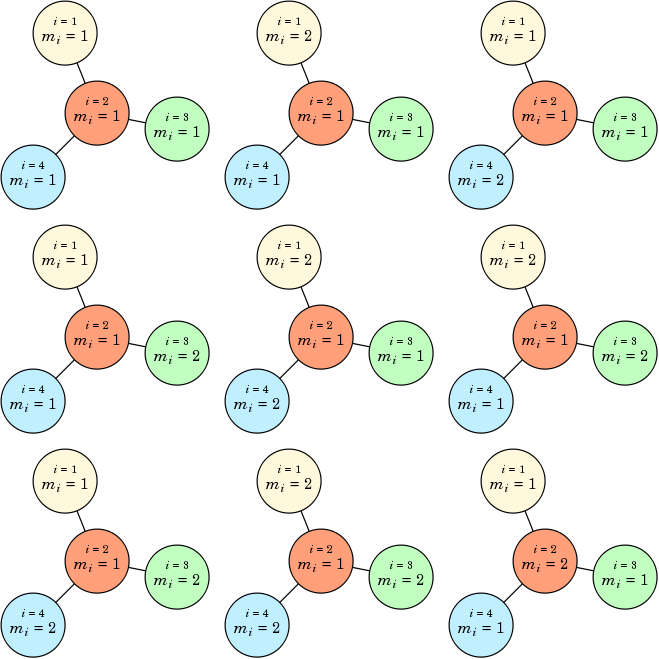
\includegraphics[width=0.9\linewidth]{figures/coding_national_stablemolecule_03.png}
    \end{center}
\end{fullwidth}

\subsection*{\sectionfont\upshape Second Data Example}
\begin{tabular}{p{0.45\linewidth}p{0.45\linewidth}}
\toprule
Example Input & Example Output \\    
\midrule
\ttfamily\setstretch{0.8}
5 3 \newline
4 2 \newline
3 2 \newline
1 3 \newline
5 3 &
\ttfamily\setstretch{0.8} 
51 \\
\bottomrule
\end{tabular}

\subsection*{\sectionfont\upshape Constraints}

โปรแกรมของคุณจะถูกทดสอบกับ test cases สองชุด (เรียกว่าชุดเล็ก และชุดใหญ่)
\begin{itemize}
\item test cases ชุดเล็กจะมีเงื่อนไขว่า ค่าขีดจำกัดสูงสุดของแรงดึดดูดระหว่างอะตอมจะสอดคล้องกับเงื่อนไข $1 \leq P \leq 10^3$
\item test cases ชุดใหญ่จะมีเงื่อนไขว่า ค่าขีดจำกัดสูงสุดของแรงดึดดูดระหว่างอะตอมจะสอดคล้องกับเงื่อนไข $1 \leq P \leq 10^9$
\item สำหรับทุก test cases จะมีเงื่อนไขว่า จำนวนของอะตอมจะสอดคล้องกับเงื่อนไข $1 \leq N \leq 1,\!000$
\end{itemize}
